%!TEX root = ../report.tex

%Citizen subscribes to service
%Sensor data is retrieved FR-1, FR-3, FR-5
%Weather data is retrieved FR-7
%Predict floud probability FR-8
%Get geo data FR-9
%The system should predict water levels FR-11, FR-12
%Monitor people should have access to a control panel FR-21

\clearpage


\section{Stories and use-cases}
This section will give an overview of the different use-cases. Figure \ref{fig:usecase-diagram} displays the use-case diagram. This provides an overview of the use-cases with their actors. In the subsections below, the architectural important use-cases are explained in more detail.

\begin{figure}[h]
\centering
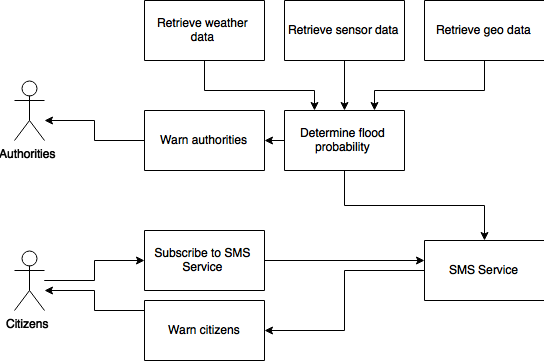
\includegraphics[bb=0 0 545 361, width=90mm]{images/usecaseDiagram.png}
\caption{Use-case diagram}
\label{fig:usecase-diagram}
\end{figure}


%slides say:
%	Name & \\
%	Number & \\
%	Primary actor &  \\
%	Scope &  \\
%	Level &  \\
%	Extensions &  \\
%	Sub-variations & \\


\subsection{Retrieve sensor data}
\pgfplotstabletypeset[%
UCTable
]{%
	value & description \\
	Number & \req{uc}\\
	Description & The system receives data from the different sensors deployed \\
	Stakeholders and interests & \compactList{itemize}{%
			\item \textbf{Developers}: Developers need to work with the sensor data
	}\\
	Primary actor & System\\
	Scope & Monitoring part of the system \\
	Level & Sub process\\
	Precondition & The sensor is connected to a processing unit \\
	Main success scenario & \compactList{enumerate}{%
			\item The sensor does a measurement
			\item The sensor sends the data to a monitoring unit
			\item The monitoring unit normalizes the received data
			\item The monitoring unit sends the normalized data to the database
			\item The database stores the data
	}\\
	Postcondition & The database received and stored the sensor data \\
	Alternatives & \compactList{itemize}{%
			\item[2a.] The data can't be sent. \\
			Data will be lost \\
			The use-case ends 
	}\\
	Related requirements & FR-1, FR-2, FR-3, FR-4, FR-5, FR-6\\
}

\clearpage

\subsection{Retrieve weather data}
\pgfplotstabletypeset[%
UCTable
]{%
	value & description \\
	Number & \req{uc}\\
	Description & The system receives data from the weather forecast service \\
	Stakeholders and interests & \compactList{itemize}{%
			\item \textbf{Developers}: Developers would like to have a simple to use API
	}\\
	Primary actor & System\\
	Scope & Monitoring part of the system \\
	Level & Sub process\\
	Precondition & The system needs external weather data to predict floods \\
	Main success scenario & \compactList{enumerate}{%
			\item The processing unit determines it needs forecast weather data%
			\item A call is made to the weather forecast service%
			\item The weather forecast service returns the requested data
	}\\
	Postcondition & The system received the forecast data \\
	Alternatives & \compactList{itemize}{%
			\item[3a.] The data can't be returned. \\
			Repeat this process with another weather forecast service. \\
			If none are available, proceed monitoring without weather forecast data. \\
			After 5 minutes try to reconnect.
	}\\
	Related requirements & FR-7\\
}

\clearpage

\subsection{Citizens subscribe to the SMS service}
\pgfplotstabletypeset[%
UCTable
]{%
	value & description \\
	Number & \req{uc}\\
	Description & Citizens can subscribe to the SMS service, so when a flood happens they will get a direct text message\\	
	Stakeholders and interests & \compactList{itemize}{
			\item \textbf{Citizens}: Citizens want to be warned as soon as possible.
	}\\
	Primary actor & Citizen\\
	Scope & Warning part of the system \\
	Level & Sub process\\
	Precondition & Citizen has a mobile phone and is not subscribed to the SMS service \\
	Main success scenario & \compactList{enumerate}{
			\item Citizen sends a text message to our service
			\item The SMS service receives the text message
			\item The SMS service stores the phone number in the database
			\item A text message is sent back to the citizen with confirmation
	}\\
	Postcondition & Citizen is subscribed to the SMS service \\
	Alternatives & \compactList{itemize}{%
			\item[2a.] The text message is not received \\
				The use-case ends
	}\\
	Related requirements & FR-16\\
}

\clearpage

\subsection{Determining flood probability}
\pgfplotstabletypeset[%
UCTable
]{%
	value & description \\
	Number & \req{uc}\\
	Description & The central processing unit calculates the probability of a flood \\
	Stakeholders and interests & \compactList{itemize}{%
			\item \textbf{Developers}: Developers have to work on this part
			\item \textbf{Emergency Services}: Emergency services want to know when a flood warning is triggered
			\item \textbf{Government}: The government would also like to know when a flood warning is triggered
	}\\
	Primary actor & System\\
	Scope & Monitoring and warning part of the system\\
	Level & Main process\\
	Precondition & The sensor data is available \\
	Main success scenario & \compactList{enumerate}{%
			\item The central processing unit gets the latest sensor data from the database
			\item The central processing unit gets the latest weather forecast data
			\item The central processing unit calculates the probabilty of a flood
			\item The central processing unit stores the probability value in the database
			\item The central processing unit determines that a flood is imminent based on the probability value
			\item A warning is send to the emergency services
			\item A warning is send to the government
			\item A warning is send to the citizens
	}\\
	Postcondition & The flood probability is calculated and stored. If the probability exceeds a certain threshold, a warning is sent to the authorities and citizens \\
	Alternatives & \compactList{itemize}{
			\item[5a.] The probability is not above the threshold \\
			The use-case ends
	}\\
	Related requirements & FR-8\\
}

\clearpage

\subsection{Warn citizens in case of an imminent flood}
\pgfplotstabletypeset[%
UCTable
]{%
	value & description \\
	Number & \req{uc}\\
	Description & Citizens who are subscribed to the SMS service will be warned through text messages in case of an imminent flood\\	
	Stakeholders and interests & \compactList{itemize}{
			\item \textbf{Citizens}: When they are subscribed, they want to warned in case of an imminent flood
	}\\
	Primary actor & Citizen\\
	Scope & Warning part of the system \\
	Level & Sub process\\
	Precondition & There is an imminent flood and citizen is subscribed to the SMS service\\
	Main success scenario & \compactList{enumerate}{%
			\item The processing unit sends a warning about an imminent flood to the SMS service 
			\item The SMS service composes a list with phone numbers to warn
			\item The SMS service sends a warning to all phone numbers on the list
	}\\
	Postcondition & The citizens who are subscribed received a warning\\
	Alternatives & \compactList{itemize}{%
			\item[3a.] A message can't be sent to the citizen \\
				Wait a minute and resend\\
				The use-case ends
	}\\
	Related requirements & FR-17\\
}

\clearpage

\subsection{Warn authorities and emergency services in case of an imminent flood}
\pgfplotstabletypeset[%
UCTable
]{%
	value & description \\
	Number & \req{uc}\\
	Description & Government and emergency services receive a warning about an imminent flood\\
	Stakeholders and interests & \compactList{itemize}{%
			\item \textbf{Government}: The government wants to warn the citizens in case of a flood
			\item \textbf{Emergency services}: The emergency services want to help the citizens in case of a flood
	}\\
	Primary actor & Government, Emergency services\\
	Scope & Warning part of the system \\
	Level & Sub process\\
	Precondition & There is an imminent flood\\
	Main success scenario & \compactList{enumerate}{
			\item The processing unit determines what area will be under water in case of a flood
			\item The processing unit determines how many people will be affected by the imminent flood
			\item The processing unit predicts how the flood will develop in the following period 
			\item The processing unit will create a map based on the current state and predictions
			\item The processing unit sends the map to the government and emergency services
	}\\
	Postcondition & A map with current and predicted data is sent to the government and emergency authorities \\
	Related requirements & FR-10, FR-11, FR-12, FR-13, FR-14 \\
}

% %\todo{joris: "The sensors send their data to the processing unit" is removed here, but is the first mss item in the preview usecases}
% \pgfplotstabletypeset[%
% UCTable
% ]{%
% 	value & description \\
% 	Number & \req{uc}\\
% 	Name & Guide citizens\\
% 	Description & A citizen requests guidance to get to a safe place in a flooded area \\
% 	Stakeholders and interests & \compactList{itemize}{%
% 			\item \textbf{Citizens}: Citizens want to be guided to a safe place in case of a flood
% 			\item \textbf{Emergency services}: The emergency services want to help the citizens in times of need}\\
% 	Primary actor & Citizen\\
% 	Scope & Guidance part of the system \\
% 	Level & Main process\\
% 	Precondition & There is a flood and the citizen is subscribed to the warning service. \\
% 	Main success scenario & \compactList{enumerate}{%
% 			\item The processing unit determined there is a flood%
% 			\item The processing unit determines generic routes
% 			\item The processing unit turns this routes into a MMS message with the right directions
% 			\item The generic routes are send through MMS message to all subscribed phone numbers}\\
% 	Postcondition & Citizen received his/her personal route to safety \\
% 	Extensions & \compactList{itemize}{%
% 			\item[4a.] MMS message can't be send. Wait a minute and try to resend}\\
% 	%Sub-variations & \\
% }

%If we decide to use user input
% \subsection{A citizen reports an obstruction}
% \textbf{Scope:} Monitoring part of the system\\\\
% \textbf{Level:} Main process\\\\
% \textbf{Primary actor:} Citizen\\\\
% \textbf{Stakeholders and interests:}\\
% 	1. Citizen - A citizen wants to report an obstruction to make the guidance part more reliable. \\\\
% \textbf{Preconditions:} There is an obstruction which is not yet reported. \\
% \textbf{Postconditions:} There is an obstruction which is reported by a citizen and is known in the system. \\\\
% \textbf{Main succes scenario:} \\
% 1 - There is an obstruction somewhere in the area. \\
% 2 - The citizen opens our application on his smartphone. \\
% 3 - The citizen reports the kind of obstruction and the location. \\
% 4 - The system gets the obstruction information as input. \\
% 5 - The obstruction is processed in the system and visible to other citizens. \\\\
% \textbf{Extensions:} \\
% 3a - The citizen doesn't know the location, GPS can be used in this case. If GPS doesn't work, the obstruction can't be reported. \\
% 4a - The smartphone can't send the information. In this case, the obstruciton can't be reported. 
